% !TEX program = xelatex
\documentclass[aspectratio=169,10pt]{beamer}

% ============================================================
% PACKAGES
% ============================================================
\usepackage{fontspec}
\usepackage{amsmath,amssymb}
\usepackage{booktabs}
\usepackage{graphicx}
\usepackage{tikz}
\usetikzlibrary{shapes.geometric, arrows.meta, positioning, calc, fit, backgrounds}
\usepackage{listings}
\usepackage{algpseudocode}
\usepackage{algorithm}
\usepackage{xcolor}
\usepackage{hyperref}
\usepackage{multicol}
\usepackage{adjustbox}
\usepackage{tabularx}
\usepackage{multirow}

% ============================================================
% THEME & COLORS
% ============================================================
\usetheme{Madrid}
\usecolortheme{whale}

% Custom colors
\definecolor{pitblue}{RGB}{31,78,121}
\definecolor{alertred}{RGB}{192,57,43}
\definecolor{successgreen}{RGB}{39,174,96}
\definecolor{warnambr}{RGB}{243,156,18}
\definecolor{codebg}{RGB}{245,245,250}
\definecolor{lightgray}{RGB}{230,230,235}
\definecolor{darkblue}{RGB}{20,50,90}

\setbeamercolor{frametitle}{bg=pitblue,fg=white}
\setbeamercolor{title}{bg=pitblue,fg=white}
\setbeamercolor{block title}{bg=pitblue,fg=white}
\setbeamercolor{block body}{bg=codebg}
\setbeamercolor{block title alerted}{bg=alertred,fg=white}
\setbeamercolor{block title example}{bg=successgreen,fg=white}

% ============================================================
% LISTING STYLE
% ============================================================
\lstdefinestyle{pseudo}{
  backgroundcolor=\color{codebg},
  basicstyle=\ttfamily\scriptsize,
  keywordstyle=\color{pitblue}\bfseries,
  commentstyle=\color{gray}\itshape,
  stringstyle=\color{successgreen},
  numbers=none,
  frame=single,
  framerule=0.3pt,
  rulecolor=\color{lightgray},
  breaklines=true,
  xleftmargin=4pt,
  xrightmargin=4pt,
  aboveskip=4pt,
  belowskip=2pt,
  columns=flexible,
  morekeywords={for,if,else,return,def,import,while,in,not,and,or,None,True,False,break,continue},
}

% ============================================================
% TITLE
% ============================================================
\title[NFP Predictor]{NFP Predictor Pipeline}
\subtitle{Institutional-Grade Non-Farm Payrolls Forecasting\\with Point-in-Time Correctness}
\author{Dhruv Kohli}
\date{\today}
\institute{}

\begin{document}

% ============================================================
\begin{frame}[plain]
\titlepage
\end{frame}

% ============================================================
\begin{frame}{Agenda}
\begin{columns}[T]
\begin{column}{0.48\textwidth}
\tableofcontents[sections={1-5}]
\end{column}
\begin{column}{0.48\textwidth}
\tableofcontents[sections={6-9}]
\end{column}
\end{columns}
\end{frame}

% ============================================================
\section{The Problem}
% ============================================================

\begin{frame}{What Are Non-Farm Payrolls?}
\begin{itemize}
  \item The \textbf{U.S. Non-Farm Payrolls (NFP)} report is the single most-watched economic release globally
  \item Published by the \textbf{Bureau of Labor Statistics (BLS)} on the first Friday of each month
  \item Measures the \textbf{month-over-month change} in total non-farm employment (thousands)
  \item Two variants:
  \begin{itemize}
    \item \textbf{NSA} (Non-Seasonally Adjusted): Raw count with calendar effects intact
    \item \textbf{SA} (Seasonally Adjusted): BLS removes recurring seasonal patterns
  \end{itemize}
  \item Our target: predict the \textbf{once-revised MoM change} (from the M+1 FRED snapshot)
\end{itemize}

\vspace{0.3cm}
\begin{block}{Target Definition}
\[
y_{\text{mom}}^{(t)} = \text{NFP}_{t}^{\text{revised}} - \text{NFP}_{t-1}^{\text{revised}}
\]
where $\text{NFP}_{t}^{\text{revised}}$ is the once-revised employment level from the $M{+}1$ vintage.
\end{block}
\end{frame}

% ============================================================
\begin{frame}{Why This Is Hard: Four Structural Challenges}
\begin{columns}[T]
\begin{column}{0.48\textwidth}
\begin{alertblock}{1. Aggressive Revisions}
BLS initial releases are heavily revised in subsequent months. Training on ``finalized'' data creates \textbf{lookahead bias}: assuming access to clean data that didn't exist in real-time.
\end{alertblock}

\vspace{0.2cm}
\begin{alertblock}{2. Asynchronous Availability}
Indicators arrive at different frequencies (daily, weekly, monthly) with varying lags:
\begin{itemize}
  \item FRED employment: $\sim$5 days
  \item ADP: $\sim$2 days before NFP
  \item NOAA storm data: $\sim$75 days late
\end{itemize}
\end{alertblock}
\end{column}
\begin{column}{0.48\textwidth}
\begin{alertblock}{3. Regime Non-Stationarity}
Economic relationships break during crises. Relationships stable during the Great Moderation (pre-2008) decoupled or \textbf{inverted} during GFC and COVID.
\end{alertblock}

\vspace{0.2cm}
\begin{alertblock}{4. High-Dimensional Instability}
\begin{itemize}
  \item $p \gg n$ problem: 49{,}000+ features vs.\ $\sim$1{,}000 rows
  \item Thousands of spurious correlations
  \item Standard ML will catastrophically overfit
\end{itemize}
\end{alertblock}
\end{column}
\end{columns}
\end{frame}

% ============================================================
\section{System Architecture}
% ============================================================

\begin{frame}{Five-Phase Architecture}
\begin{center}
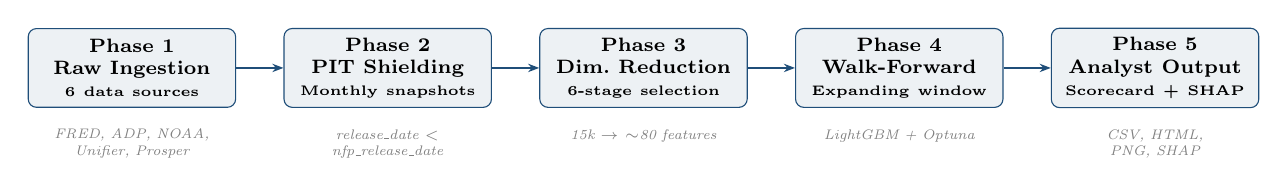
\begin{tikzpicture}[
  node distance=0.5cm and 0.3cm,
  phase/.style={rectangle, rounded corners=3pt, draw=pitblue, fill=pitblue!8, text width=2.4cm, minimum height=1.0cm, align=center, font=\scriptsize\bfseries},
  arrow/.style={-{Stealth[length=4pt]}, thick, pitblue},
  lbl/.style={font=\tiny\itshape, text=gray, align=center, text width=2.4cm},
]
  \node[phase] (ingest) {Phase 1\\Raw Ingestion\\{\tiny 6 data sources}};
  \node[phase, right=0.6cm of ingest] (pit) {Phase 2\\PIT Shielding\\{\tiny Monthly snapshots}};
  \node[phase, right=0.6cm of pit] (fs) {Phase 3\\Dim.\ Reduction\\{\tiny 6-stage selection}};
  \node[phase, right=0.6cm of fs] (train) {Phase 4\\Walk-Forward\\{\tiny Expanding window}};
  \node[phase, right=0.6cm of train] (out) {Phase 5\\Analyst Output\\{\tiny Scorecard + SHAP}};

  \draw[arrow] (ingest) -- (pit);
  \draw[arrow] (pit) -- (fs);
  \draw[arrow] (fs) -- (train);
  \draw[arrow] (train) -- (out);

  \node[lbl, below=0.15cm of ingest] {FRED, ADP, NOAA, Unifier, Prosper};
  \node[lbl, below=0.15cm of pit] {release\_date $<$ nfp\_release\_date};
  \node[lbl, below=0.15cm of fs] {15k $\to$ $\sim$80 features};
  \node[lbl, below=0.15cm of train] {LightGBM + Optuna};
  \node[lbl, below=0.15cm of out] {CSV, HTML, PNG, SHAP};
\end{tikzpicture}
\end{center}

\vspace{0.2cm}
\begin{columns}[T]
\begin{column}{0.32\textwidth}
\begin{block}{Data Sources}
\scriptsize
\begin{itemize}
  \item 159 FRED employment series
  \item 10 FRED exogenous indicators
  \item ADP private payrolls
  \item NOAA storm damage data
  \item 11 Unifier/LSEG indicators
  \item Prosper consumer surveys
\end{itemize}
\end{block}
\end{column}
\begin{column}{0.32\textwidth}
\begin{block}{Selection Pipeline}
\scriptsize
\begin{itemize}
  \item Stage 0: Variance filter
  \item Stage 1: Dual filter (corr + LightGBM)
  \item Stage 2: Boruta shadow features
  \item Stage 3: Vintage stability
  \item Stage 4: Cluster redundancy
  \item Stages 5--6: Optional (SFS)
\end{itemize}
\end{block}
\end{column}
\begin{column}{0.32\textwidth}
\begin{block}{Training}
\scriptsize
\begin{itemize}
  \item Expanding window backtest
  \item Dynamic reselection (every 24mo)
  \item Optuna composite tuning
  \item NSA: 5-stage enhancement
  \item SA: enhancement exempt
  \item Kalman + AccelOverride fusion
\end{itemize}
\end{block}
\end{column}
\end{columns}
\end{frame}

% ============================================================
\section{Point-in-Time Correctness}
% ============================================================

\begin{frame}{The Fundamental Constraint}
\begin{block}{Point-in-Time Rule (Applies Everywhere)}
\[
\forall\; \text{feature } X_i \text{ mapped to month } t: \quad
\texttt{feature\_release\_date}(X_i) \;<\; \texttt{nfp\_release\_date}(t)
\]
\textbf{Strict inequality} ($<$, not $\le$): data published on the exact NFP release day is \emph{excluded}.
\end{block}

\vspace{0.3cm}
\begin{columns}[T]
\begin{column}{0.55\textwidth}
\begin{exampleblock}{PIT Enforcement by Source}
\footnotesize
\begin{tabular}{@{}lp{5.5cm}@{}}
\toprule
\textbf{Source} & \textbf{Mechanism} \\
\midrule
FRED Empl. & ALFRED vintage \texttt{realtime\_start} \\
FRED Exog. & NFP-windowed weekly aggregation \\
ADP & \texttt{release\_date < nfp\_release\_date} \\
NOAA & month-end + 75 day lag model \\
Unifier & Median lag repair for missing \texttt{first\_release\_date} \\
Prosper & \texttt{release\_date < nfp\_release\_date} \\
\bottomrule
\end{tabular}
\end{exampleblock}
\end{column}
\begin{column}{0.42\textwidth}
\begin{alertblock}{The Unifier Bug}
\footnotesize
When \texttt{first\_release\_date} is missing, Unifier fills \texttt{last\_revision\_date} with \emph{today's timestamp}---making 2015 data appear available today.

\textbf{Fix:} Compute per-series \texttt{median\_lag\_days} from valid observations, use that instead. Never trust \texttt{last\_revision\_date} when \texttt{first\_release\_date} is NULL.
\end{alertblock}
\end{column}
\end{columns}
\end{frame}

% ============================================================
\begin{frame}[fragile]{PIT: Weekly Data Aggregation}
\begin{block}{Problem}
Weekly claims data (CCNSA, CCSA) cannot be aggregated by calendar month---some weeks span month boundaries, and claims published \emph{after} the NFP release would leak.
\end{block}

\vspace{0.2cm}
\begin{block}{Solution: NFP-Windowed Bucketing}
\begin{lstlisting}[style=pseudo]
def aggregate_weekly_to_monthly_nfp_based(weekly_df, nfp_map):
    for each month M:
        nfp_prev = nfp_release_date(M - 1)
        nfp_curr = nfp_release_date(M)
        # Only include data RELEASED between prev and curr NFP
        mask = (weekly_df.release_date >= nfp_prev) &
               (weekly_df.release_date <  nfp_curr)
        monthly_agg[M] = weekly_df[mask].mean()
    return monthly_agg
\end{lstlisting}
\end{block}

\vspace{0.1cm}
\footnotesize
A claim reported on January 15\textsuperscript{th} (after the January 10\textsuperscript{th} NFP release) goes into \textbf{February's bucket}---matching what an analyst would actually have in hand.
\end{frame}

% ============================================================
\begin{frame}[fragile]{PIT: FRED Release Date Imputation}
For historical data where \texttt{realtime\_start} is unavailable (pre-2009), two strategies:

\vspace{0.2cm}
\begin{columns}[T]
\begin{column}{0.48\textwidth}
\begin{block}{Simple (First-Release Files)}
\begin{lstlisting}[style=pseudo]
def impute_simple(month):
    # First Friday of the month
    day_1 = date(year, month, 1)
    weekday = day_1.weekday()
    offset = (4 - weekday) % 7  # Friday
    return day_1 + offset
\end{lstlisting}
\end{block}
\end{column}
\begin{column}{0.48\textwidth}
\begin{block}{Complex (Last-Release Files)}
3-tier gate system:
\begin{itemize}\footnotesize
  \item \textbf{Option 1:} Extended backfill for very old data (pre-2009, no metadata)
  \item \textbf{Option 2:} Intermediate backfill for partial metadata
  \item \textbf{Option 3:} Closest candidate respecting snapshot timing
\end{itemize}
\end{block}
\end{column}
\end{columns}
\end{frame}

% ============================================================
\section{Data Sources}
% ============================================================

\begin{frame}{Data Source Overview}
\begin{center}
\footnotesize
\begin{tabular}{@{}lllrl@{}}
\toprule
\textbf{Source} & \textbf{API / Origin} & \textbf{Frequency} & \textbf{Features} & \textbf{History} \\
\midrule
FRED Employment  & FRED / ALFRED & Monthly & $\sim$11{,}600 & $\sim$1948 \\
FRED Exogenous   & FRED + Yahoo Finance & Daily/Weekly & $\sim$50 & $\sim$1990 \\
ADP Employment   & investing.com & Monthly & $\sim$15 & $\sim$2001 \\
NOAA Storm Events & NCEI (gzip CSV) & Event-level & $\sim$30 & $\sim$1996 \\
Unifier / LSEG   & Unifier API & Monthly & $\sim$100 & varies \\
Prosper Surveys  & Prosper API & Monthly & $\sim$200 & $\sim$2009 \\
\midrule
\textbf{Total}   & & & $\sim$\textbf{15{,}500} & \\
\bottomrule
\end{tabular}
\end{center}

\vspace{0.2cm}
\begin{itemize}\footnotesize
  \item All sources produce monthly \textbf{PIT-safe parquet snapshots} stored in decade-based directory structure
  \item Path convention: \texttt{base\_dir/decades/\{decade\}s/\{year\}/YYYY-MM.parquet}
  \item Feature count after ETL-time feature selection: $\sim$15{,}000 (all-features mode; selection deferred to training)
\end{itemize}
\end{frame}

% ============================================================
\begin{frame}{FRED Employment: 159-Series Hierarchy}
\begin{columns}[T]
\begin{column}{0.45\textwidth}
\begin{center}
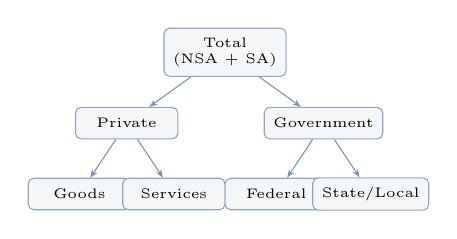
\begin{tikzpicture}[
  level distance=0.9cm,
  sibling distance=1.6cm,
  every node/.style={rectangle, rounded corners=2pt, draw=pitblue!50, fill=pitblue!5, font=\tiny, minimum width=1.3cm, minimum height=0.4cm, align=center},
  edge from parent/.style={draw=pitblue!60, -{Stealth[length=3pt]}},
  level 1/.style={sibling distance=2.5cm},
  level 2/.style={sibling distance=1.2cm},
]
  \node {Total\\(NSA + SA)}
    child { node {Private}
      child { node {Goods} }
      child { node {Services} }
    }
    child { node {Government}
      child { node {Federal} }
      child { node {State/Local} }
    };
\end{tikzpicture}
\end{center}
\vspace{0.1cm}
\footnotesize
Full hierarchy extends 7 levels deep into sub-industries (Manufacturing, Construction, Mining, Health Care, Leisure, etc.)
\end{column}
\begin{column}{0.52\textwidth}
\begin{block}{9 Features Per Series ($\times$ 159 Series = 1{,}431)}
\footnotesize
\begin{tabular}{@{}ll@{}}
\toprule
\textbf{Feature} & \textbf{Formula} \\
\midrule
\texttt{\_latest} & Raw level $L_t$ \\
\texttt{\_MoM} & $L_t - L_{t-1}$ \\
\texttt{\_MoM\_pct} & $(L_t - L_{t-1}) / L_{t-1}$ \\
\texttt{\_3m} & $L_t - L_{t-3}$ \\
\texttt{\_6m} & $L_t - L_{t-6}$ \\
\texttt{\_YoY} & $L_t - L_{t-12}$ \\
\texttt{\_12m\_pct} & $(L_t - L_{t-12}) / L_{t-12}$ \\
\texttt{\_rolling\_3m} & $\frac{1}{3}\sum_{k=0}^{2} \Delta L_{t-k}$ \\
\texttt{\_volatility} & $\text{std}(\Delta L_{t:t-2})$ \\
\bottomrule
\end{tabular}
\end{block}
\footnotesize
Data sourced via \textbf{ALFRED vintage API} to preserve \texttt{realtime\_start} metadata for PIT correctness.
\end{column}
\end{columns}
\end{frame}

% ============================================================
\begin{frame}{FRED Exogenous: Financial \& Macro Indicators}
\begin{columns}[T]
\begin{column}{0.52\textwidth}
\begin{block}{10 Indicator Series}
\scriptsize
\begin{tabular}{@{}lll@{}}
\toprule
\textbf{Series} & \textbf{FRED ID} & \textbf{Signal} \\
\midrule
Credit Spreads & BAMLH0A0HYM2 & Risk appetite \\
Yield Curve & T10Y2Y & Recession proxy \\
Oil Prices & DCOILWTICO & Energy sector \\
VIX & VIXCLS & Market fear \\
S\&P 500 & Yahoo Finance & Equity market \\
Fin.\ Stress & STLFSI4 & Systemic risk \\
Econ.\ Index & WEI & Weekly GDP proxy \\
Claims (NSA) & CCNSA & Labor slack \\
Claims (SA) & CCSA & Labor slack \\
Ind.\ Prod & --- & Output signal \\
\bottomrule
\end{tabular}
\end{block}
\end{column}
\begin{column}{0.45\textwidth}
\begin{block}{Binary Regime Indicators}
\scriptsize
\emph{NOT differenced}---binary nature makes transforms meaningless:
\begin{itemize}
  \item \texttt{VIX\_panic\_regime}: VIX $> 40$
  \item \texttt{VIX\_high\_regime}: VIX $> 25$
  \item \texttt{SP500\_bear\_market}: drawdown $> 20\%$
  \item \texttt{SP500\_crash\_month}: return $< -10\%$
  \item \texttt{SP500\_circuit\_breaker}: drop $> 7\%$
\end{itemize}
\end{block}
\vspace{0.1cm}
\begin{exampleblock}{API Resilience}
\scriptsize
Exponential backoff: 2s, 4s, 8s. Thread-safe rate limit: 0.8s/request.
\end{exampleblock}
\end{column}
\end{columns}
\end{frame}

% ============================================================
\begin{frame}{ADP, NOAA, Unifier, Prosper}
\begin{columns}[T]
\begin{column}{0.48\textwidth}
\begin{block}{ADP Employment}
\footnotesize
\begin{itemize}
  \item Source: investing.com REST API
  \item Private-sector payroll change (thousands)
  \item Independent from BLS establishment survey
  \item PIT: \texttt{release\_date < nfp\_release\_date}
  \item Features: \texttt{pct\_change} + lean \texttt{compute\_all\_features} (no symlog)
\end{itemize}
\end{block}
\vspace{0.15cm}
\begin{block}{NOAA Storm Events}
\footnotesize
\begin{itemize}
  \item CPI-adjusted property \& crop damage
  \item State$\to$national: \textbf{employment-weighted} aggregation
  \item 75-day lag after month-end (NCEI processing)
  \item Hurricane in Texas (large employment) $>$ same storm in Wyoming
\end{itemize}
\end{block}
\end{column}
\begin{column}{0.48\textwidth}
\begin{block}{Unifier / LSEG (11 Indicators)}
\footnotesize
\begin{itemize}
  \item ISM Mfg \& Non-Mfg, Consumer Confidence
  \item Housing Starts, Retail Sales, Industrial Production
  \item Avg Weekly Hours, Avg Hourly Earnings
  \item Empire State Mfg, UMich Expectations
  \item \textbf{NFP Consensus Poll} (economists' mean forecast)
  \item Zero-centered handling for Empire State
\end{itemize}
\end{block}
\vspace{0.15cm}
\begin{block}{Prosper Consumer Surveys}
\footnotesize
\begin{itemize}
  \item Consumer Mood, Spending Forecast
  \item Employment expectations by demographic
  \item \textbf{Historical break fix:} Pre-9/2009 ``employed'' question split into FT+PT post-9/2009; merged into continuous series
\end{itemize}
\end{block}
\end{column}
\end{columns}
\end{frame}

% ============================================================
\begin{frame}{Feature Transforms: The SymLog \& Derived Feature Chain}
\begin{columns}[T]
\begin{column}{0.55\textwidth}
\begin{block}{Transform Chain (Applied Per Source)}
\footnotesize
\begin{enumerate}
  \item \texttt{add\_symlog\_copies()}: $\text{symlog}(x) = \text{sign}(x) \cdot \ln(1 + |x|)$
  \item \texttt{add\_pct\_change\_copies()}: $\Delta\% = \frac{x_t - x_{t-1}}{x_{t-1}} \times 100$
  \item \texttt{compute\_all\_features()}: Lags, rolling stats, momentum
\end{enumerate}
\end{block}

\begin{block}{Derived Features Per Series (Full Mode)}
\scriptsize
\begin{tabular}{@{}ll@{}}
\toprule
\textbf{Feature} & \textbf{Formula} \\
\midrule
\texttt{level} & $x_t$ \\
\texttt{diff} & $x_t - x_{t-1}$ \\
\texttt{diff\_zscore\_3m} & $(x_t - \bar{x}_{3m}) / \sigma_{3m}$ \\
\texttt{diff\_zscore\_12m} & $(x_t - \bar{x}_{12m}) / \sigma_{12m}$ \\
\texttt{zscore\_3m/12m} & Rolling z-score of level \\
\texttt{rolling\_mean\_3m} & $\frac{1}{3}\sum_{k=0}^{2} x_{t-k}$ \\
\texttt{rolling\_std\_6m} & $\sigma(x_{t:t-5})$ \\
\texttt{chg\_3m/6m/12m} & $x_t - x_{t-k}$ \\
\texttt{lag\_1/3/6/12m} & $x_{t-k}$ \\
\bottomrule
\end{tabular}
\end{block}
\end{column}
\begin{column}{0.42\textwidth}
\begin{exampleblock}{Why SymLog?}
\footnotesize
\begin{itemize}
  \item Standard log undefined for negatives
  \item SymLog handles \emph{both} signs
  \item Preserves zero values: $\text{symlog}(0) = 0$
  \item Compresses extreme kurtosis
  \item On NFP MoM data: skewness $-6.5 \to -1.1$, kurtosis $81 \to -0.7$
\end{itemize}
\end{exampleblock}

\vspace{0.15cm}
\begin{alertblock}{Lean Mode (ADP, etc.)}
\footnotesize
Skip symlog (tree-invariant for monotonic transforms). Keep only: level, pct\_chg, diff, diff\_zscore\_3m, rolling stats, chg\_{3,6,12}m.
\end{alertblock}
\end{column}
\end{columns}
\end{frame}

% ============================================================
\begin{frame}{Revision Features: Capturing Data Revision Dynamics}
\begin{block}{Motivation}
\footnotesize
When BLS revises prior months' data, the \emph{pattern} of revisions contains signal---systematic upward revisions suggest strengthening, while large revision volatility suggests measurement uncertainty.
\end{block}

\vspace{0.2cm}
\begin{columns}[T]
\begin{column}{0.48\textwidth}
\begin{block}{6 Aggregate Revision Features}
\scriptsize
\begin{tabular}{@{}lp{4.5cm}@{}}
\toprule
\textbf{Feature} & \textbf{Formula} \\
\midrule
\texttt{rev\_mean} & $\bar{r} = \text{mean}(S_t^{(M)} - S_t^{(M-1)})$ \\
\texttt{rev\_abs\_mean} & $\text{mean}(|r_i|)$ \\
\texttt{rev\_positive\_ratio} & $\text{mean}(r_i > 0)$ \\
\texttt{rev\_count} & $\#\{r_i \ne 0\}$ \\
\texttt{rev\_max\_abs} & $\max(|r_i|)$ \\
\texttt{rev\_std} & $\text{std}(r_i)$ \\
\bottomrule
\end{tabular}
\end{block}
\end{column}
\begin{column}{0.48\textwidth}
\begin{block}{Construction}
\scriptsize
For target month $M$:
\begin{enumerate}
  \item Load snapshot at $M$ and snapshot at $M{-}1$
  \item Restrict both to observations \textbf{before} $M{-}1$ cutoff (no lookahead)
  \item Compute: $r_i = \text{snap}_M[i] - \text{snap}_{M-1}[i]$
  \item Aggregate into 6 statistics
\end{enumerate}
\end{block}
\end{column}
\end{columns}
\end{frame}

% ============================================================
\section{Feature Selection Engine}
% ============================================================

\begin{frame}{Feature Selection: The 7-Stage Pipeline}
\begin{center}
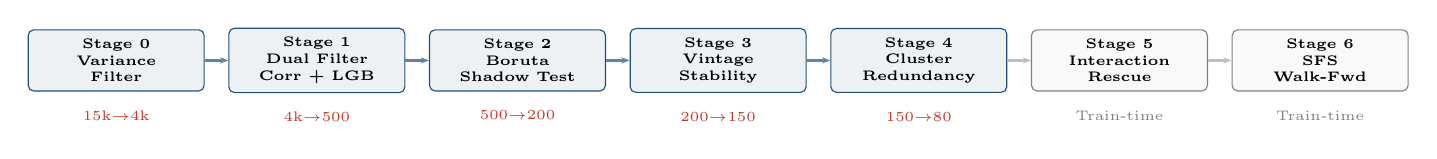
\begin{tikzpicture}[
  stage/.style={rectangle, rounded corners=2pt, draw=pitblue, fill=pitblue!8, text width=2.0cm, minimum height=0.65cm, align=center, font=\tiny\bfseries},
  arrow/.style={-{Stealth[length=3pt]}, thick, pitblue!70},
  countlbl/.style={font=\tiny\color{alertred}},
]
  \node[stage] (s0) {Stage 0\\Variance\\Filter};
  \node[stage, right=0.3cm of s0] (s1) {Stage 1\\Dual Filter\\Corr + LGB};
  \node[stage, right=0.3cm of s1] (s2) {Stage 2\\Boruta\\Shadow Test};
  \node[stage, right=0.3cm of s2] (s3) {Stage 3\\Vintage\\Stability};
  \node[stage, right=0.3cm of s3] (s4) {Stage 4\\Cluster\\Redundancy};
  \node[stage, right=0.3cm of s4, draw=gray, fill=gray!5] (s5) {Stage 5\\Interaction\\Rescue};
  \node[stage, right=0.3cm of s5, draw=gray, fill=gray!5] (s6) {Stage 6\\SFS\\Walk-Fwd};

  \draw[arrow] (s0) -- (s1);
  \draw[arrow] (s1) -- (s2);
  \draw[arrow] (s2) -- (s3);
  \draw[arrow] (s3) -- (s4);
  \draw[arrow, gray!50] (s4) -- (s5);
  \draw[arrow, gray!50] (s5) -- (s6);

  \node[countlbl, below=0.12cm of s0] {15k$\to$4k};
  \node[countlbl, below=0.12cm of s1] {4k$\to$500};
  \node[countlbl, below=0.12cm of s2] {500$\to$200};
  \node[countlbl, below=0.12cm of s3] {200$\to$150};
  \node[countlbl, below=0.12cm of s4] {150$\to$80};
  \node[font=\tiny\color{gray}, below=0.12cm of s5] {Train-time};
  \node[font=\tiny\color{gray}, below=0.12cm of s6] {Train-time};
\end{tikzpicture}
\end{center}

\vspace{0.2cm}
\begin{columns}[T]
\begin{column}{0.55\textwidth}
\begin{block}{Default Pipeline: Stages (0, 1, 2, 3, 4)}
\footnotesize
\begin{itemize}
  \item Runs \textbf{independently per source} and \textbf{per regime}
  \item $\sim$5 min per source
  \item Results cached with 30-day TTL
  \item Stages 5--6: used in dynamic reselection at train time
\end{itemize}
\end{block}
\end{column}
\begin{column}{0.42\textwidth}
\begin{exampleblock}{Stage Presets}
\scriptsize
\begin{tabular}{@{}ll@{}}
\toprule
\textbf{Preset} & \textbf{Stages} \\
\midrule
Default & (0,1,2,3,4) \\
Fast & (0,1,4) \\
Fast+Vintage & (0,1,3,4) \\
Fast+Boruta & (0,1,2,4) \\
Full & (0,1,2,3,4,5,6) \\
\bottomrule
\end{tabular}
\end{exampleblock}
\end{column}
\end{columns}
\end{frame}

% ============================================================
\begin{frame}[fragile]{Stage 0: Variance Filter + Spearman Pre-Screen}
\begin{columns}[T]
\begin{column}{0.48\textwidth}
\begin{block}{Variance Filter}
\footnotesize
Remove features where $\ge 97\%$ of non-NaN values are identical.

\textbf{Two-tier approach} (for efficiency on 17k+ features):
\begin{enumerate}
  \item \textbf{Tier 1 (fast):} \texttt{nunique()} classification
  \begin{itemize}\scriptsize
    \item $\text{nunique} \le 1$: constant $\to$ \textbf{drop}
    \item $\text{nunique} > 5$: variable $\to$ \textbf{keep}
    \item $\text{nunique} \in [2,5]$: ambiguous
  \end{itemize}
  \item \textbf{Tier 2 (exact):} \texttt{np.unique()} per ambiguous column; compute mode frequency
\end{enumerate}
Minimum 30 non-NaN values required per column.
\end{block}
\end{column}
\begin{column}{0.48\textwidth}
\begin{block}{Spearman Pre-Screen ($p > 5{,}000$)}
\footnotesize
When source has $> 5{,}000$ features (FRED Employment at $\sim$17k):

\begin{enumerate}
  \item Compute vectorized Spearman $\rho$ with target
  \item Apply Benjamini--Hochberg FDR correction at $\alpha = 0.30$
  \item Drop features with $p_{\text{adj}} > 0.30$
\end{enumerate}

\textbf{Effect:} Reduces Stage 1 input by $\sim$78\%, cutting runtime from $\sim$10 min to $\sim$2 min with zero empirical signal loss.
\end{block}
\end{column}
\end{columns}
\end{frame}

% ============================================================
\begin{frame}[fragile]{Stage 1: Dual Filter}
\begin{columns}[T]
\begin{column}{0.48\textwidth}
\begin{block}{A) Purged Expanding Correlation}
\footnotesize
Expanding windows with \textbf{3-month purge gap}:
\[
\bar{\rho} = \frac{\sum_k \sqrt{n_k} \cdot |\rho_k|}{\sum_k \sqrt{n_k}}
\]
where $\rho_k$ = Spearman correlation in window $k$, $n_k$ = window size.

\textbf{Purge:} 3-month gap between training and evaluation prevents information leakage.

\textbf{Deduplication} via hierarchical clustering:
\begin{itemize}\scriptsize
  \item Spearman threshold: $0.95$
  \item Agglomerative with average linkage
  \item Chunked for $> 5{,}000$ features (2-phase: local$\to$merge with shuffling)
\end{itemize}
\end{block}
\end{column}
\begin{column}{0.48\textwidth}
\begin{block}{B) Random Subspace LightGBM}
\footnotesize
Captures \textbf{non-linear importance} that correlation misses:
\begin{lstlisting}[style=pseudo]
for each random subspace:
    X_sub = random_sample(features, k)
    model = LightGBM(X_sub, y)
    importance[X_sub] += model.gain
# Rank by cumulative importance
\end{lstlisting}

\vspace{0.1cm}
LightGBM parameters:
\begin{itemize}\scriptsize
  \item \texttt{objective}: regression (L2)
  \item \texttt{n\_estimators}: 100
  \item \texttt{num\_leaves}: 31
  \item \texttt{n\_jobs}: 1 (macOS OOM safety)
\end{itemize}
\end{block}
\end{column}
\end{columns}
\end{frame}

% ============================================================
\begin{frame}{Stages 2--4: Boruta, Vintage Stability, Cluster Redundancy}
\begin{columns}[T]
\begin{column}{0.32\textwidth}
\begin{block}{Stage 2: Boruta}
\footnotesize
Shadow-feature permutation test (100 runs):
\begin{enumerate}\scriptsize
  \item Create ``shadow'' features by shuffling each real feature
  \item Train LightGBM on real + shadow
  \item Record max shadow importance
  \item Feature ``confirmed'' if it beats shadow max in statistically significant number of runs (binomial test)
\end{enumerate}
\textbf{Guard:} Max 500 features input.
\end{block}
\end{column}
\begin{column}{0.32\textwidth}
\begin{block}{Stage 3: Vintage Stability}
\footnotesize
Reject features with unstable predictive power across regimes.

\textbf{6 Hard-coded regimes:}
\begin{enumerate}\scriptsize
  \item Pre-GFC (1998)
  \item GFC Shock (2008)
  \item Late-Cycle (2015)
  \item COVID (2020-03)
  \item Inflation (2022-03)
  \item AI/Trump (2025-02)
\end{enumerate}
Exponential recency weighting. Default lookback: 3 months (NOAA: 6).
\end{block}
\end{column}
\begin{column}{0.32\textwidth}
\begin{block}{Stage 4: Cluster Redundancy}
\footnotesize
Collapse collinear survivors:
\begin{enumerate}\scriptsize
  \item \textbf{NaN-aware} Spearman correlation (pairwise non-NaN overlap)
  \item Hierarchical clustering
  \item Keep one representative per cluster (highest target correlation)
\end{enumerate}
\textbf{Key:} NaN-awareness handles different start dates (FRED $\sim$1948, ADP $\sim$2001, Prosper $\sim$2009).
\end{block}
\end{column}
\end{columns}
\end{frame}

% ============================================================
\begin{frame}{Master Snapshot Aggregation}
\begin{columns}[T]
\begin{column}{0.52\textwidth}
\begin{block}{7 Source Directories $\to$ 1 Wide Parquet Per Month}
\scriptsize
\begin{tabular}{@{}ll@{}}
\toprule
\textbf{Source Key} & \textbf{Exec Order} \\
\midrule
FRED\_Employment\_NSA & 1st (longest) \\
FRED\_Employment\_SA & 2nd \\
FRED\_Exogenous & 3rd \\
Unifier & 4th \\
Prosper & 5th \\
NOAA & 6th \\
ADP & 7th (fastest) \\
\bottomrule
\end{tabular}
\end{block}

\vspace{0.1cm}
\begin{block}{Target Combos}
\footnotesize
\begin{tabular}{@{}lll@{}}
\toprule
\textbf{Target Type} & \textbf{Source} & \textbf{FS Target Mode} \\
\midrule
NSA & revised & \texttt{mom} \\
SA & revised & \texttt{model\_aligned} \\
\bottomrule
\end{tabular}
\end{block}
\end{column}
\begin{column}{0.45\textwidth}
\begin{block}{All-Features Mode (Current)}
\footnotesize
Master snapshots store \textbf{all} lean features ($\sim$15{,}500 per month). No ETL-time selection.

\vspace{0.1cm}
Feature selection is entirely deferred to \textbf{train-time dynamic reselection} (2-pass Boruta + cluster redundancy), which selects $\sim$80 features per backtest window.

\vspace{0.1cm}
\textbf{Advantage:} Every feature is re-evaluated with current data---no permanent information loss from stale ETL decisions.
\end{block}

\vspace{0.1cm}
\begin{exampleblock}{Caching Architecture}
\scriptsize
\begin{itemize}
  \item \textbf{Source cache:} per source, 30-day TTL
  \item \textbf{Regime cache:} per cutoff month, 30-day TTL
  \item \textbf{Branch cache:} per target config, 30-day TTL
  \item Version: \texttt{2026-02-24-regime-cache-v1}
\end{itemize}
\end{exampleblock}
\end{column}
\end{columns}
\end{frame}

% ============================================================
\section{Training Pipeline}
% ============================================================

\begin{frame}[fragile]{Expanding Window Backtest: The Core Loop}
\begin{lstlisting}[style=pseudo]
for target_month in [oldest_backtest_month, ..., latest]:
    # 1. Expanding window: data strictly before target
    X_train, y_train = load_data(before=target_month)

    # 2. Feature engineering (parallel via joblib)
    X_train += calendar_features(target_month)
    X_train += lagged_target_features(y_train)
    X_train += revision_features(target_month)

    # 3. Dynamic reselection (every 24 months, 2-pass)
    if months_since_reselection >= 24:
        features = dynamic_reselect(X_train, y_train)  # max 80

    # 4. Optuna tuning (every 12 months, composite objective)
    if months_since_tune >= 12:
        params = optuna_tune(X_train, y_train, target_month)

    # 5. Train LightGBM (85/15 chronological split)
    model = train_lgbm(X_train[features], y_train, params)

    # 6. Variance enhancement (NSA: full stack; SA: exempt)
    prediction = enhance(model, X_test, enhancements)

    # 7. Record result
    results.append(prediction, actual, intervals, baselines)
\end{lstlisting}
\end{frame}

% ============================================================
\begin{frame}{Feature Engineering: Calendar \& Survey Week Features}
\begin{columns}[T]
\begin{column}{0.48\textwidth}
\begin{block}{Cyclical Encoding}
\footnotesize
Preserves December $\to$ January proximity (superior to one-hot for trees):
\begin{align*}
\texttt{month\_sin} &= \sin\!\left(\frac{2\pi \cdot m}{12}\right) \\
\texttt{month\_cos} &= \cos\!\left(\frac{2\pi \cdot m}{12}\right) \\
\texttt{quarter\_sin} &= \sin\!\left(\frac{2\pi \cdot q}{4}\right) \\
\texttt{quarter\_cos} &= \cos\!\left(\frac{2\pi \cdot q}{4}\right)
\end{align*}
\end{block}

\begin{alertblock}{SA Calendar Filtering}
\scriptsize
SA series have seasonality stripped by BLS. Only keep: \texttt{weeks\_since\_last\_survey}, \texttt{is\_5\_week\_month}, \texttt{year}.
\end{alertblock}
\end{column}
\begin{column}{0.48\textwidth}
\begin{block}{BLS Survey Week Logic}
\footnotesize
NFP reference week = pay period containing the \textbf{12th of the month}.

\begin{enumerate}\scriptsize
  \item Find the 12th of the month
  \item Find the Sunday of that week (survey week start)
  \item Compute gap to previous month's survey week:
\end{enumerate}
\[
\texttt{weeks} = \lfloor (\text{survey}_t - \text{survey}_{t-1}) / 7 \rfloor
\]
Result: \textbf{4 or 5 weeks}. A 5-week interval allows more accumulated job growth/loss, systematically inflating NSA counts.
\end{block}

\begin{block}{Other Features}
\scriptsize
\begin{itemize}
  \item \texttt{is\_jan}: BLS seasonal factor refresh
  \item \texttt{is\_july}: Mid-year benchmark revision
  \item \texttt{year}: Secular trend
\end{itemize}
\end{block}
\end{column}
\end{columns}
\end{frame}

% ============================================================
\begin{frame}[fragile]{Dynamic Feature Selection (2-Pass)}
\begin{block}{When master snapshots store ALL features (\texttt{mode: "all\_features"})}
\footnotesize
Dynamic reselection is the sole feature selection path during the backtest.
\end{block}

\vspace{0.2cm}
\begin{columns}[T]
\begin{column}{0.48\textwidth}
\begin{block}{Pass 1: Per-Source (Stages 0,2,4,5)}
\begin{lstlisting}[style=pseudo]
for source in [FRED_NSA, FRED_SA,
               FRED_Exog, Unifier,
               ADP, NOAA, Prosper]:
    survivors[source] = run_fs(
        X_train[source_cols],
        y_train,
        stages=(0, 2, 4, 5)
    )
\end{lstlisting}
\end{block}
\end{column}
\begin{column}{0.48\textwidth}
\begin{block}{Pass 2: Global (Stages 0,1,2,4)}
\begin{lstlisting}[style=pseudo]
all_survivors = union(survivors.values())
all_survivors += target_derived_features
all_survivors += calendar_features

final = run_fs(
    X_train[all_survivors],
    y_train,
    stages=(0, 1, 2, 4),
    max_features=50  # hard cap
)
\end{lstlisting}
\end{block}
\end{column}
\end{columns}

\vspace{0.2cm}
\begin{exampleblock}{Parameters}
\scriptsize
Reselection frequency: every 24 months (configurable). NaN eval window: post-2010. Max NaN rate: 20\%.
Sample weighting: uniform (no recency decay)---selects features with durable long-term signal.
\end{exampleblock}
\end{frame}

% ============================================================
\begin{frame}[fragile]{Dynamic Feature Selection: All-Features Mode}
\begin{columns}[T]
\begin{column}{0.48\textwidth}
\begin{block}{All-Features Mode}
\footnotesize
Master snapshots store \textbf{all 15{,}497 lean features}. No ETL-time pruning. Feature selection is entirely deferred to the 2-pass dynamic reselection during the backtest.

\vspace{0.15cm}
\textbf{Advantages:}
\begin{itemize}\scriptsize
  \item Every feature gets a fresh evaluation each window
  \item No permanent information loss from ETL decisions
  \item Adapts to structural regime changes
\end{itemize}
\end{block}

\begin{block}{Uniform Sample Weighting}
\footnotesize
Equal weight across all history (no recency decay). Selects features with \textbf{durable, long-term predictive power} rather than recent-month noise.
\[
w_i = 1 \quad \forall\; i \quad \text{(uniform)}
\]
Jaccard stability: 0.976--0.979 between windows.
\end{block}
\end{column}
\begin{column}{0.48\textwidth}
\begin{block}{Branch-Target: Dynamics Composite (SA)}
\footnotesize
Multi-signal ranking for variance capture:
\begin{align*}
S &= 0.25 \cdot |\rho(X,y)| & \text{Level}\\
  &+ 0.25 \cdot |\rho(\Delta X, \Delta y)| & \text{Diff}\\
  &+ 0.15 \cdot \tanh\!\left(\frac{|\mu_{\uparrow}{-}\mu_{\downarrow}|}{\sqrt{\sigma^2}}\right) & \text{Direction}\\
  &+ 0.20 \cdot |\rho(|\Delta X|, |\Delta y|)| & \text{Magnitude}\\
  &+ 0.10 \cdot \text{sign\_agree} & \text{Sign}\\
  &+ 0.05 \cdot \text{tail\_align} & \text{Tail}
\end{align*}
\end{block}
\footnotesize
NSA: uses simple \texttt{weighted\_corr} (top 8). SA: uses dynamics composite (top 20).
\end{column}
\end{columns}
\end{frame}

% ============================================================
\begin{frame}{Sample Weighting: Exponential Decay + Tail Awareness}
\begin{columns}[T]
\begin{column}{0.48\textwidth}
\begin{block}{Exponential Decay}
\footnotesize
Recent observations weighted higher:
\[
w_i = \exp\!\left(-\frac{\ln 2 \cdot d_i}{h}\right)
\]
where:
\begin{itemize}\scriptsize
  \item $d_i = (\text{target\_month} - \text{date}_i) / 30.44$ (months)
  \item $h \in [12, 120]$ months (tuned by Optuna)
  \item Normalized: $w \leftarrow w / \bar{w}$
\end{itemize}

\textbf{Interpretation:} With $h = 60$ months, data from 5 years ago has weight $= 0.5$; data from 10 years ago has weight $= 0.25$.
\end{block}
\end{column}
\begin{column}{0.48\textwidth}
\begin{block}{Tail-Aware Boosting (Variance Targets)}
\footnotesize
Prevents the model from ignoring large moves:
\begin{align*}
m_i &= 1.0 \quad \text{(base)} \\
\text{if } |y_i| &\ge Q_{0.80}(|y|): \quad m_i \mathrel{*}= 1.35 \\
\text{if } |\Delta y_i| &\ge Q_{0.80}(|\Delta y|): \quad m_i \mathrel{*}= 1.35 \\
m_i &\leftarrow \text{clip}(m_i,\; 1.0,\; 2.50) \\
w_i^{\text{final}} &= w_i^{\text{decay}} \cdot m_i
\end{align*}
Observations with both extreme level AND extreme change get up to $2.5\times$ weight boost.
\end{block}
\end{column}
\end{columns}
\end{frame}

% ============================================================
\begin{frame}[fragile]{LightGBM Training: CV + Final Model}
\begin{columns}[T]
\begin{column}{0.48\textwidth}
\begin{block}{Training Process}
\begin{lstlisting}[style=pseudo]
# Phase 1: 5-fold TimeSeriesSplit CV
for fold in TimeSeriesSplit(n_splits=5):
    train on earlier data
    validate on later data
    accumulate OOF residuals

# Phase 2: Final model
train_size = 85% of data
X_train, X_val = split(X, 0.85)
model = lgb.train(
    params,
    train_data,
    num_boost_round=1000,
    early_stopping=50,
    valid_sets=[val_data]
)
# Extract gain importance + residuals
\end{lstlisting}
\end{block}
\end{column}
\begin{column}{0.48\textwidth}
\begin{block}{Why LightGBM?}
\footnotesize
\begin{itemize}
  \item \textbf{Native NaN handling:} Split-finder tries both branches for missing values, choosing whichever reduces loss more
  \item Critical for staggered datasets where FRED starts $\sim$1948 but Prosper starts $\sim$2009
  \item No imputation = no artificial patterns
  \item \texttt{inf} replaced with NaN (LightGBM handles NaN but not inf)
\end{itemize}
\end{block}

\begin{block}{Default Parameters}
\scriptsize
\begin{tabular}{@{}lr@{}}
\toprule
\texttt{objective} & regression \\
\texttt{metric} & mae \\
\texttt{learning\_rate} & 0.03 \\
\texttt{num\_leaves} & 31 \\
\texttt{max\_depth} & 6 \\
\texttt{feature\_fraction} & 0.8 \\
\texttt{bagging\_fraction} & 0.8 \\
\bottomrule
\end{tabular}
\end{block}
\end{column}
\end{columns}
\end{frame}

% ============================================================
\begin{frame}{Hyperparameter Tuning: Leakage-Safe Optuna}
\begin{columns}[T]
\begin{column}{0.48\textwidth}
\begin{block}{Architecture}
\footnotesize
\begin{itemize}
  \item \textbf{Inner TimeSeriesSplit} (5 folds) within each outer expanding window step
  \item Outer backtest: data $< t$
  \item Inner CV: further splits into train/val
  \item No future data ever leaks
\end{itemize}
\end{block}

\begin{block}{Optimization Config}
\scriptsize
\begin{tabular}{@{}ll@{}}
\toprule
Sampler & TPE (seed=42) \\
Pruner & Median (10 startup, 20 warmup) \\
Budget & 25 trials, 300s timeout \\
Frequency & Every 12 backtest months \\
Warm-start & Previous best $\to$ Trial 0 \\
\bottomrule
\end{tabular}
\end{block}
\end{column}
\begin{column}{0.48\textwidth}
\begin{block}{Search Space}
\scriptsize
\begin{tabular}{@{}lll@{}}
\toprule
\textbf{Parameter} & \textbf{Range} & \textbf{Scale} \\
\midrule
learning\_rate & [0.005, 0.15] & Log \\
num\_leaves & [15, 127] & Linear \\
max\_depth & [3, 8] & Linear \\
min\_data\_in\_leaf & [1, 50] & Linear \\
feature\_fraction & [0.4, 1.0] & Linear \\
bagging\_fraction & [0.5, 1.0] & Linear \\
$\lambda_{L1}$ & [$10^{-8}$, 10] & Log \\
$\lambda_{L2}$ & [$10^{-8}$, 10] & Log \\
half\_life (months) & [12, 120] & Linear \\
huber\_delta & [25, 500] & Linear \\
\bottomrule
\end{tabular}
\end{block}
\end{column}
\end{columns}
\end{frame}

% ============================================================
\section{Variance Enhancement Stack}
% ============================================================

\begin{frame}{Variance Enhancement: 5-Stage Sequential Stack}
\begin{center}
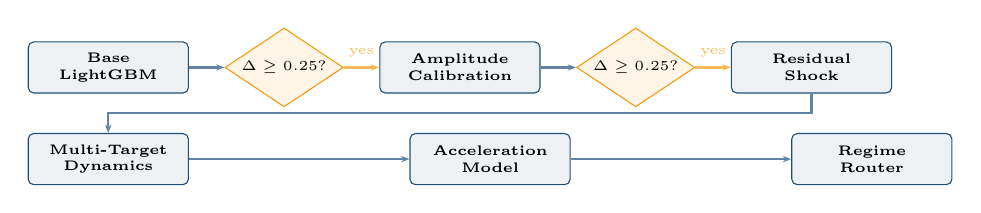
\begin{tikzpicture}[
  stage/.style={rectangle, rounded corners=2pt, draw=pitblue, fill=pitblue!8, text width=1.8cm, minimum height=0.65cm, align=center, font=\tiny\bfseries},
  gate/.style={diamond, draw=warnambr, fill=warnambr!10, aspect=1.5, font=\tiny, inner sep=1pt},
  arrow/.style={-{Stealth[length=3pt]}, thick, pitblue!70},
  gatearrow/.style={-{Stealth[length=3pt]}, thick, warnambr!70},
]
  \node[stage] (base) {Base\\LightGBM};
  \node[gate, right=0.45cm of base] (g1) {$\Delta \ge 0.25$?};
  \node[stage, right=0.45cm of g1] (amp) {Amplitude\\Calibration};
  \node[gate, right=0.45cm of amp] (g2) {$\Delta \ge 0.25$?};
  \node[stage, right=0.45cm of g2] (shock) {Residual\\Shock};
  \node[stage, below=0.5cm of base] (dyn) {Multi-Target\\Dynamics};
  \node[stage, right=2.8cm of dyn] (accel) {Acceleration\\Model};
  \node[stage, right=2.8cm of accel] (regime) {Regime\\Router};

  \draw[arrow] (base) -- (g1);
  \draw[gatearrow] (g1) -- node[above, font=\tiny\color{successgreen}]{yes} (amp);
  \draw[arrow] (amp) -- (g2);
  \draw[gatearrow] (g2) -- node[above, font=\tiny\color{successgreen}]{yes} (shock);
  \draw[arrow] (shock) |- ([yshift=-0.25cm]shock.south) -| (dyn);
  \draw[arrow] (dyn) -- (accel);
  \draw[arrow] (accel) -- (regime);
\end{tikzpicture}
\end{center}

\vspace{0.15cm}
\begin{columns}[T]
\begin{column}{0.48\textwidth}
\begin{block}{Gate Rule}
\footnotesize
Each stage is kept \textbf{only if} it improves the composite validation score by $\ge 0.25$. Otherwise, the prediction from the previous stage is carried forward.
\end{block}
\end{column}
\begin{column}{0.48\textwidth}
\begin{block}{Enhancement Sequences}
\footnotesize
\begin{itemize}
  \item \textbf{NSA:} Full stack (amplitude $\to$ shock $\to$ dynamics $\to$ acceleration $\to$ regime)
  \item \textbf{SA:} Enhancement exempt (base LightGBM predictions---amplitude calibration tested but degraded recent performance)
\end{itemize}
\end{block}
\end{column}
\end{columns}
\end{frame}

% ============================================================
\begin{frame}{Enhancement Details: Amplitude, Shock, Dynamics}
\begin{columns}[T]
\begin{column}{0.32\textwidth}
\begin{block}{A: Amplitude Calibration}
\footnotesize
\[
\hat{y}_{\text{cal}} = a + b \cdot \hat{y}
\]
where $(a, b) = \text{polyfit}(\hat{y}_{\text{val}},\; y_{\text{val}},\; 1)$

\vspace{0.1cm}
Slope clamped: $b \in [0.50, 3.00]$

\vspace{0.1cm}
Min samples: 12

\vspace{0.1cm}
\textbf{Purpose:} Correct systematic under/over-prediction of magnitude.
\end{block}
\end{column}
\begin{column}{0.32\textwidth}
\begin{block}{B: Residual Shock}
\footnotesize
Separate shallow LightGBM on residual errors:
\begin{itemize}\scriptsize
  \item max\_depth: 3
  \item num\_leaves: 15
  \item 200 boosting rounds
\end{itemize}

\vspace{0.1cm}
If residuals have structure (e.g., larger during high-VIX), this captures it.

\[
\hat{y}_{\text{shock}} = \hat{y}_{\text{cal}} + f_{\text{shock}}(X)
\]
\end{block}
\end{column}
\begin{column}{0.32\textwidth}
\begin{block}{C: Multi-Target Dynamics}
\footnotesize
Three sub-models:
\begin{itemize}\scriptsize
  \item \textbf{Magnitude:} $|\Delta \hat{y}|$
  \item \textbf{Direction:} $P(\Delta y > 0)$
  \item \textbf{Level:} Current best $\hat{y}$
\end{itemize}
\begin{align*}
\delta_c &= 0.7 \delta_{\text{mag}} + 0.3 \delta_{\text{cur}} \\
c &= |p - 0.5| \\
b &= \min(0.8 c,\; 1) \\
\delta_f &= (1{-}b)\delta_c + b\delta_{\text{dir}}
\end{align*}
Min confidence: $|p - 0.5| > 0.12$
\end{block}
\end{column}
\end{columns}
\end{frame}

% ============================================================
\begin{frame}{Enhancement Details: Acceleration \& Regime Router}
\begin{columns}[T]
\begin{column}{0.48\textwidth}
\begin{block}{D: Acceleration Model}
\footnotesize
Train on the ``change of change'' target:
\[
y_{\text{accel}}^{(t)} = y^{(t)} - y^{(t-1)}
\]
Separate shallow LightGBM (depth=3, leaves=15, 200 rounds).

\vspace{0.15cm}
\textbf{Reconstruction:}
\[
\hat{y}^{(t)} = y^{(t-1)} + \hat{y}_{\text{accel}}^{(t)}
\]

\vspace{0.15cm}
\textbf{Motivation:} Captures momentum dynamics that the level model misses. If NFP has been accelerating (increasing MoM), this model detects it.
\end{block}
\end{column}
\begin{column}{0.48\textwidth}
\begin{block}{E: Regime Router}
\footnotesize
\textbf{Partition} training data by target volatility:
\begin{itemize}\scriptsize
  \item Low-vol: $|y| < Q_{0.75}(|y|)$
  \item High-vol: $|y| \ge Q_{0.75}(|y|)$
\end{itemize}

\vspace{0.1cm}
\textbf{Train} separate expert LightGBMs for each regime.

\vspace{0.1cm}
\textbf{Router:} Logistic classifier predicts $P(\text{high-vol})$.

\vspace{0.1cm}
\textbf{Soft blend:}
\[
\hat{y} = (1 - p_h) \cdot \hat{y}_{\text{low}} + p_h \cdot \hat{y}_{\text{high}}
\]

Min 20 samples per regime required.
\end{block}
\end{column}
\end{columns}
\end{frame}

% ============================================================
\section{Metrics \& Evaluation}
% ============================================================

\begin{frame}{Variance Capture Metrics}
\begin{block}{The Problem: Variance Collapse}
\footnotesize
Standard metrics (RMSE, MAE) can mask a critical failure: the model predicts the general trend but \textbf{flattens month-to-month amplitude}. The prediction series has lower standard deviation than the actual.
\end{block}

\vspace{0.2cm}
\begin{center}
\scriptsize
\begin{tabular}{@{}llcl@{}}
\toprule
\textbf{Metric} & \textbf{Formula} & \textbf{Target} & \textbf{Interpretation} \\
\midrule
$\text{STD Ratio}$ & $\sigma(\hat{y}) / \sigma(y)$ & $1.0$ & $< 1$ means flattening \\
$\text{Diff STD Ratio}$ & $\sigma(\Delta\hat{y}) / \sigma(\Delta y)$ & $1.0$ & MoM acceleration amplitude \\
$\rho_{\text{level}}$ & $\text{corr}(y, \hat{y})$ & $> 0.8$ & Overall trend following \\
$\rho_{\text{diff}}$ & $\text{corr}(\Delta y, \Delta \hat{y})$ & $> 0.6$ & Change-of-change tracking \\
$\text{Diff Sign Acc}$ & $\mathbb{E}[\text{sign}(\Delta y) = \text{sign}(\Delta \hat{y})]$ & $> 0.65$ & Direction of change \\
$\text{Tail MAE}$ & $\mathbb{E}[|e|; |y| \ge Q_{0.75}]$ & minimize & Error on large moves \\
$\text{Extreme Hit}$ & $P(|\hat{y}| \ge Q_{0.90} \mid |y| \ge Q_{0.90})$ & $> 0.60$ & Extreme event recall \\
\bottomrule
\end{tabular}
\end{center}
\end{frame}

% ============================================================
\begin{frame}{Composite Objective Function}
\begin{block}{Used by Optuna Tuning (\texttt{objective\_mode = 'composite'}) for SA Targets}
\begin{align*}
\mathcal{L}_{\text{composite}} = \;&\text{MAE} \\
  &+ 25.0 \cdot |1 - \text{STD Ratio}| \\
  &+ 25.0 \cdot |1 - \text{Diff STD Ratio}| \\
  &+ 0.20 \cdot \text{Tail MAE} \\
  &+ 20.0 \cdot (1 - \rho_{\text{diff}}) \\
  &+ 12.0 \cdot (1 - \text{Diff Sign Accuracy}) \\
  &+ 15.0 \cdot (1 - \text{Acceleration Accuracy}) \\
  &+ 10.0 \cdot (1 - \text{Directional Accuracy})
\end{align*}
\end{block}

\vspace{0.1cm}
\begin{columns}[T]
\begin{column}{0.48\textwidth}
\begin{exampleblock}{Variance Promotion Gates (SA)}
\scriptsize
\begin{tabular}{@{}lr@{}}
\toprule
\textbf{Gate} & \textbf{Minimum} \\
\midrule
STD Ratio & 0.60 \\
Diff STD Ratio & 0.45 \\
$\rho_{\text{diff}}$ & 0.25 \\
Diff Sign Accuracy & 0.55 \\
Extreme Hit Rate & 0.25 \\
\bottomrule
\end{tabular}
\end{exampleblock}
\end{column}
\begin{column}{0.48\textwidth}
\begin{block}{Directional Accuracy}
\footnotesize
Two complementary metrics:
\begin{align*}
\text{dir\_correct} &= \mathbb{1}[\text{sign}(y) = \text{sign}(\hat{y})] \\
\text{accel\_correct} &= \mathbb{1}[\text{sign}(\Delta y) = \text{sign}(\Delta \hat{y})]
\end{align*}
where $\Delta y_t = y_t - y_{t-1}$ (acceleration).
\end{block}
\end{column}
\end{columns}
\end{frame}

% ============================================================
\begin{frame}{Prediction Intervals \& Baselines}
\begin{columns}[T]
\begin{column}{0.48\textwidth}
\begin{block}{Non-Parametric Confidence Intervals}
\footnotesize
No Gaussian assumption. Purely empirical from historical OOS residuals:
\[
\text{CI}_{\alpha} = \left[\hat{y} + Q_{\alpha/2}(r),\;\; \hat{y} + Q_{1-\alpha/2}(r)\right]
\]
where $r = \{y_i - \hat{y}_i\}$ are historical residuals.

\vspace{0.15cm}
\textbf{Coverage levels:} 50\%, 80\%, 95\%

\vspace{0.15cm}
Requires $\ge 10$ residuals. For forward predictions, uses up to last 36 OOS residuals.
\end{block}
\end{column}
\begin{column}{0.48\textwidth}
\begin{block}{Naive Baselines}
\footnotesize
Computed \textbf{per backtest step} using only training data:

\vspace{0.1cm}
\textbf{Last-$y$:} $\hat{y}_{\text{base}} = y_{t-1}$ (random walk)

\vspace{0.1cm}
\textbf{Rolling Mean:} $\hat{y}_{\text{base}} = \frac{1}{6}\sum_{k=1}^{6} y_{t-k}$
\end{block}

\begin{alertblock}{Keep Rule}
\footnotesize
If trailing 12-month MAE exceeds best baseline:
\begin{itemize}\scriptsize
  \item Action: \texttt{skip\_save} (don't deploy model)
  \item Tolerance: 0.0 (must beat baseline)
  \item Window: 12 months trailing OOS
\end{itemize}
\end{alertblock}
\end{column}
\end{columns}
\end{frame}

% ============================================================
\section{Model Variants \& Output}
% ============================================================

\begin{frame}{Model Variants \& Output Structure}
\begin{columns}[T]
\begin{column}{0.48\textwidth}
\begin{block}{2 Model Variants (Default)}
\footnotesize
\begin{tabular}{@{}llp{3cm}@{}}
\toprule
\textbf{ID} & \textbf{Target} & \textbf{Purpose} \\
\midrule
\texttt{nsa\_first\_revised} & NSA & Once-revised NSA MoM \\
\texttt{sa\_first\_revised} & SA & Once-revised SA MoM \\
\bottomrule
\end{tabular}

\vspace{0.1cm}
Revised target: MoM from M+1 FRED snapshot (once-revised).

\vspace{0.1cm}
\texttt{predict\_nfp\_mom()} enforces \texttt{operational\_available\_date} checks at inference.
\end{block}

\begin{block}{Consensus Anchor (Post-Training)}
\footnotesize
\begin{itemize}
  \item \textbf{Kalman Fusion:} State-space model fusing consensus + model
  \item \textbf{Accel Override:} Consensus base + model momentum
  \item Both PIT-safe (min 12 months history)
\end{itemize}
\end{block}
\end{column}
\begin{column}{0.48\textwidth}
\begin{block}{Output Artifacts (\texttt{\_output/})}
\scriptsize
\begin{tabular}{@{}lp{4.3cm}@{}}
\toprule
\textbf{Folder} & \textbf{Contents} \\
\midrule
\texttt{NSA\_prediction/} & Backtest CSV, predictions PNG, SHAP, feature importance, summary stats \\
\texttt{SA\_prediction/} & Same structure \\
\texttt{NSA\_plus\_adjustment/} & NSA + exp-weighted seasonal adjustment vs actual SA \\
\texttt{Predictions/} & Forward predictions with 50/80/95\% CIs \\
\texttt{models/lightgbm\_nfp/} & Saved models + comparison scorecard (CSV + HTML) \\
\texttt{Archive/} & Timestamped snapshots \\
\bottomrule
\end{tabular}
\end{block}
\end{column}
\end{columns}
\end{frame}

% ============================================================
\section{Operations \& Reproducibility}
% ============================================================

\begin{frame}[fragile]{Running the Pipeline}
\begin{columns}[T]
\begin{column}{0.48\textwidth}
\begin{block}{Full Pipeline}
\begin{lstlisting}[style=pseudo, morekeywords={python,bash}]
# End-to-end
python run_full_project.py

# Fresh re-download
python run_full_project.py --fresh

# Individual stages
python run_full_project.py --stage data
python run_full_project.py --stage train
python run_full_project.py --stage train --no-tune

# Skip sources
python run_full_project.py --skip noaa,prosper
\end{lstlisting}
\end{block}
\end{column}
\begin{column}{0.48\textwidth}
\begin{block}{Direct Training}
\begin{lstlisting}[style=pseudo, morekeywords={python}]
# All variants + scorecard
python Train/train_lightgbm_nfp.py --train-all

# Single variant
python Train/train_lightgbm_nfp.py --train \
  --target sa --release first

# Production inference
python scripts/predict_next_nfp.py --target nsa
\end{lstlisting}
\end{block}

\begin{block}{Environment Overrides}
\begin{lstlisting}[style=pseudo]
# Fast feature selection
NFP_FS_STAGES="0,1,4" python run_full_project.py

# Enable performance profiling
NFP_PERF=1 python run_full_project.py
\end{lstlisting}
\end{block}
\end{column}
\end{columns}
\end{frame}

% ============================================================
\begin{frame}{Economic Shock Handling \& Reproducibility}
\begin{columns}[T]
\begin{column}{0.48\textwidth}
\begin{block}{COVID Winsorization}
\footnotesize
\begin{itemize}
  \item Spring 2020 extremes clipped to non-COVID quantiles (1st/99th percentile)
  \item Applied \textbf{per-fold} during backtest (not globally)
  \item Model doesn't ``know'' COVID happened until it reaches March 2020
  \item Preserves directional information
\end{itemize}
\end{block}

\begin{block}{SymLog Transform}
\footnotesize
\[
\text{symlog}(x) = \text{sign}(x) \cdot \ln(1 + |x|)
\]
\begin{itemize}\scriptsize
  \item Handles both positive and negative values
  \item Compresses extreme kurtosis
  \item $\text{symlog}(0) = 0$ (preserves zero)
  \item Inverse: $\text{sign}(y) \cdot (e^{|y|} - 1)$
\end{itemize}
\end{block}
\end{column}
\begin{column}{0.48\textwidth}
\begin{block}{Post-1990 Data Floor}
\footnotesize
\texttt{DATA\_START\_FLOOR = 1990-01-01}

Pre-1990 data is extremely sparse for non-FRED sources and degrades feature selection quality.
\end{block}

\vspace{0.2cm}
\begin{exampleblock}{Reproducibility}
\footnotesize
\begin{itemize}
  \item \textbf{Seeds:} LightGBM \texttt{random\_state=42}, Optuna TPE \texttt{seed=42}
  \item \textbf{Determinism:} Expanding-window splits are strictly chronological, no shuffling
  \item \textbf{Tracking:} Perf profiling JSONs in \texttt{\_temp/perf/}
  \item \textbf{Archiving:} Output snapshots in \texttt{\_output/Archive/}
  \item \textbf{CI:} pytest + ruff + mypy across Python 3.10--3.12
\end{itemize}
\end{exampleblock}
\end{column}
\end{columns}
\end{frame}

% ============================================================
\section{Consensus Anchor Fusion}
% ============================================================

\begin{frame}{Consensus Anchor: Kalman Filter Fusion}
\begin{columns}[T]
\begin{column}{0.52\textwidth}
\begin{block}{State-Space Model (3-Channel Information Filter)}
\footnotesize
\textbf{State:} $x_t$ = true SA NFP MoM (random walk)
\begin{align*}
\text{Prior:} \quad x_t^- &= x_{t-1}, \quad P_t^- = P_{t-1} + Q \\
\text{Update:} \quad P_t &= \left(\frac{1}{P_t^-} + \frac{1}{R_c} + \frac{1}{R_m} + \frac{w_a}{R_a}\right)^{-1} \\
x_t &= P_t \left(\frac{x_t^-}{P_t^-} + \frac{z_c}{R_c} + \frac{z_m}{R_m} + \frac{w_a z_a}{R_a}\right)
\end{align*}
where:
\begin{itemize}\scriptsize
  \item $z_c$ = consensus prediction, $R_c$ = trailing consensus error variance
  \item $z_m$ = model channel ($R_m$ = trailing error variance):
    \begin{itemize}\tiny
      \item Model A: SA Direct LightGBM
      \item Model B: NSA+Adjustment
    \end{itemize}
  \item $z_a$ = NSA+Adj acceleration channel (Model A only)
  \item $w_a$ = NSA weight scale (Optuna-tuned)
\end{itemize}
\end{block}
\end{column}
\begin{column}{0.45\textwidth}
\begin{block}{Optuna Tuning (Composite Objective)}
\footnotesize
\[
\mathcal{L} = \text{MAE} - 50 \cdot \text{AccelAcc} - 30 \cdot \text{DirAcc}
\]
Tunable parameters:
\begin{itemize}\scriptsize
  \item \texttt{trailing\_window} $\in [6, 36]$ months
  \item \texttt{nsa\_weight\_scale} $\in [0.1, 3.0]$
\end{itemize}
\textbf{Tuned values:} $\text{tw}=28$, $w_a=1.84$
\end{block}

\begin{block}{AccelOverride (Direction Correction)}
\footnotesize
Majority vote on acceleration direction using consensus + SA blend + NSA+Adj signals. If majority disagrees with consensus direction:
\[
\hat{y} = y_{t-1} + \text{dir}_{\text{majority}} \cdot |z_c - y_{t-1}|
\]
Tuned: $\kappa = 0.40$, mode = ``consensus''
\end{block}
\end{column}
\end{columns}
\end{frame}

% ============================================================
\section{Results}
% ============================================================

\begin{frame}{Backtest Results: NSA Model (60-Month OOS)}
\begin{center}
\includegraphics[width=0.95\textwidth]{_output/presentation/nsa_backtest.png}
\end{center}
\vspace{-0.2cm}
\footnotesize
\begin{itemize}
  \item 60-month expanding window backtest (2021-04 to 2026-02), model retrained from scratch each month
  \item NSA MAE: 241.6K (vs baseline last-$y$: 911.7K, rolling mean: 701.1K)
  \item 100\% directional accuracy, 88.2\% acceleration accuracy on NSA target
  \item Full enhancement stack active (amplitude, shock, dynamics, acceleration, regime)
\end{itemize}
\end{frame}

% ============================================================
\begin{frame}{Backtest Results: SA Model (60-Month OOS)}
\begin{center}
\includegraphics[width=0.95\textwidth]{_output/presentation/sa_backtest.png}
\end{center}
\vspace{-0.2cm}
\footnotesize
\begin{itemize}
  \item SA model uses separately selected features from SA master snapshots
  \item Dynamic reselection every 24 months with uniform sample weighting (no recency bias)
  \item 80 features selected per window (50 snapshot + branch-target + calendar + revision)
  \item SA enhancement: exempt from variance stack (base LightGBM predictions used directly)
\end{itemize}
\end{frame}

% ============================================================
\begin{frame}{Two Final Models: Balanced vs Precision}
\begin{center}
\includegraphics[width=0.92\textwidth]{_output/presentation/both_models_vs_consensus.png}
\end{center}
\vspace{-0.2cm}
\footnotesize
Both models use consensus-anchored Kalman fusion. They differ in which model signals feed the filter:
\begin{columns}[T]
\begin{column}{0.48\textwidth}
\begin{block}{Model A: Balanced (Blue)}
\scriptsize
3-channel: consensus + SA Direct + NSA+Adj\\
Best \textbf{acceleration accuracy} (54.3\% recent)\\
Slight MAE trade-off vs consensus
\end{block}
\end{column}
\begin{column}{0.48\textwidth}
\begin{block}{Model B: Precision (Green)}
\scriptsize
2-channel: consensus + NSA+Adj only\\
Best \textbf{MAE} and \textbf{RMSE} (95.5 / 135.5)\\
Weaker on recent acceleration (40.0\%)
\end{block}
\end{column}
\end{columns}
\end{frame}

% ============================================================
\begin{frame}{Model Comparison: Full Period \& Recent}
\begin{center}
\includegraphics[width=0.88\textwidth]{_output/presentation/metrics_comparison_dual.png}
\end{center}
\vspace{-0.2cm}
\begin{center}
\scriptsize
\begin{tabular}{@{}l|rrrr|rrrr@{}}
\toprule
& \multicolumn{4}{c|}{\textbf{Full 59 Months}} & \multicolumn{4}{c}{\textbf{Last 36 Months}} \\
\textbf{Model} & MAE & RMSE & Accel & Dir & MAE & RMSE & Accel & Dir \\
\midrule
\textbf{Model A (Balanced)} & 105.9 & 148.2 & \textbf{56.9\%} & 96.6\% & 67.1 & 84.0 & \textbf{54.3\%} & 94.4\% \\
\textbf{Model B (Precision)} & \textbf{95.5} & \textbf{135.5} & 53.4\% & 96.6\% & 67.6 & \textbf{82.3} & 40.0\% & 94.4\% \\
\rowcolor{codebg}
Consensus & 109.7 & 166.0 & 44.8\% & 96.6\% & \textbf{65.7} & 85.6 & 42.9\% & 94.4\% \\
\bottomrule
\end{tabular}
\end{center}
\end{frame}

% ============================================================
\begin{frame}{Model A: Balanced --- Best for Acceleration}
\begin{center}
\includegraphics[width=0.90\textwidth]{_output/presentation/model_a_vs_consensus.png}
\end{center}
\vspace{-0.2cm}
\footnotesize
\begin{columns}[T]
\begin{column}{0.48\textwidth}
\begin{exampleblock}{Strengths}
\begin{itemize}\scriptsize
  \item \textbf{54.3\% acceleration accuracy} on last 36m (vs 42.9\% consensus: $+$26\%)
  \item 56.9\% full-period acceleration ($+$27\% vs consensus)
  \item RMSE 148.2 ($-$10.7\% vs consensus)
\end{itemize}
\end{exampleblock}
\end{column}
\begin{column}{0.48\textwidth}
\begin{block}{Architecture}
\scriptsize
Kalman filter with 3 channels:
\begin{enumerate}
  \item Consensus (level anchor)
  \item SA Direct LightGBM (variance signal)
  \item NSA+Adjustment (acceleration signal)
\end{enumerate}
\texttt{tw=18}, \texttt{nsa\_ws=1.0}
\end{block}
\end{column}
\end{columns}
\end{frame}

% ============================================================
\begin{frame}{Model B: Precision --- Best for MAE/RMSE}
\begin{center}
\includegraphics[width=0.90\textwidth]{_output/presentation/model_b_vs_consensus.png}
\end{center}
\vspace{-0.2cm}
\footnotesize
\begin{columns}[T]
\begin{column}{0.48\textwidth}
\begin{exampleblock}{Strengths}
\begin{itemize}\scriptsize
  \item \textbf{MAE 95.5} ($-$13.0\% vs consensus)
  \item \textbf{RMSE 135.5} ($-$18.4\% vs consensus)
  \item Lowest cumulative error over full period
\end{itemize}
\end{exampleblock}
\end{column}
\begin{column}{0.48\textwidth}
\begin{block}{Architecture}
\scriptsize
Kalman filter with 2 channels:
\begin{enumerate}
  \item Consensus (level anchor)
  \item NSA+Adjustment (acceleration + level)
\end{enumerate}
\texttt{tw=18}, no SA Direct channel.\\
Simpler = more stable predictions.
\end{block}
\end{column}
\end{columns}
\end{frame}

% ============================================================
\begin{frame}{Cumulative Error: Both Models vs Consensus}
\begin{center}
\includegraphics[width=0.92\textwidth]{_output/presentation/cumulative_error_dual.png}
\end{center}
\vspace{-0.2cm}
\footnotesize
\begin{columns}[T]
\begin{column}{0.48\textwidth}
\begin{block}{Key Insight}
Both models accumulate less total error than consensus. Model B (green) has the lowest cumulative error; Model A (blue) tracks closely while capturing acceleration dynamics better.
\end{block}
\end{column}
\begin{column}{0.48\textwidth}
\begin{block}{When to Use Which}
\begin{itemize}\scriptsize
  \item \textbf{Model A:} When catching turning points and momentum shifts matters most (trading, risk)
  \item \textbf{Model B:} When minimizing absolute prediction error matters most (forecasting, planning)
\end{itemize}
\end{block}
\end{column}
\end{columns}
\end{frame}

% ============================================================
\begin{frame}{Feature Selection \& Post-Training Fusion}
\begin{columns}[T]
\begin{column}{0.48\textwidth}
\begin{block}{Dynamic Reselection Config}
\footnotesize
\begin{tabular}{@{}lr@{}}
\toprule
\textbf{Parameter} & \textbf{Value} \\
\midrule
Reselection interval & 36 months \\
Sample weighting & Uniform \\
Max features (Pass-2) & 80 \\
Total in snapshots & 15{,}497 \\
Optuna objective & Composite \\
Optuna trials & 25 per window \\
\bottomrule
\end{tabular}
\end{block}

\begin{exampleblock}{Top SA Features}
\scriptsize
\begin{enumerate}
  \item \texttt{CCSA\_monthly\_avg\_diff}
  \item \texttt{NFP\_Consensus\_Mean\_chg\_3m}
  \item \texttt{CB\_Consumer\_Confidence\_chg\_12m}
  \item \texttt{nfp\_sa\_accel\_rolling\_3m}
  \item \texttt{Financial\_Stress\_monthly\_avg}
\end{enumerate}
\end{exampleblock}
\end{column}
\begin{column}{0.48\textwidth}
\begin{block}{Post-Training Chain}
\footnotesize
\begin{enumerate}\scriptsize
  \item \textbf{NSA LightGBM} $\to$ NSA predictions (full enhancement stack)
  \item \textbf{SA LightGBM} $\to$ SA predictions (enhancement exempt, with NSA accel features)
  \item \textbf{Predicted Adjustment:} NSA pred + exp-weighted seasonal factor $\to$ NSA+Adj (SA space)
  \item \textbf{Kalman Fusion:}
    \begin{itemize}\scriptsize
      \item Model A: cons + SA + NSA+Adj
      \item Model B: cons + NSA+Adj
    \end{itemize}
  \item \textbf{Output:} Two predictions per month; user selects based on priority
\end{enumerate}
\end{block}
\end{column}
\end{columns}
\end{frame}

% ============================================================
\section{Summary}
% ============================================================

\begin{frame}{Key Design Principles}
\begin{enumerate}
  \item \textbf{Point-in-Time Above All:} Every feature satisfies $\texttt{release\_date} < \texttt{nfp\_release\_date}$. No same-day leakage. Per-source PIT fixes for FRED vintage, Unifier bugs, NOAA lags, weekly windowing.

  \item \textbf{Native NaN Handling:} LightGBM handles missing values mathematically. No imputation, no forward-fill. Different start dates across sources are tolerated.

  \item \textbf{Regime Awareness:} Feature selection tests stability across 6 macroeconomic regimes. Exponential recency weighting prioritizes recent signal.

  \item \textbf{Variance Capture:} Composite objective prevents ``variance collapse.'' 5-stage enhancement stack (amplitude, shock, dynamics, acceleration, regime). Tail-aware sample weighting for extreme events.

  \item \textbf{Expanding Window Discipline:} Model retrained from scratch each month. No K-Fold. COVID winsorization per-fold. Baseline keep-rule gating prevents deployment of models worse than naive heuristics.

  \item \textbf{Efficiency at Scale:} $p \gg n$ datasets (15k features, $\sim$430 rows) handled via random subspace selection, chunked clustering, vectorized operations, joblib parallelism, and aggressive caching.
\end{enumerate}
\end{frame}

% ============================================================
\begin{frame}{Pipeline Summary: Data $\to$ Prediction}
\begin{center}
\footnotesize
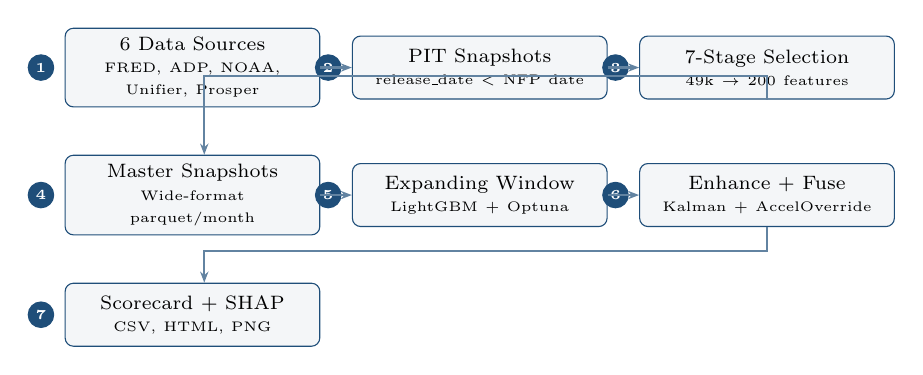
\begin{tikzpicture}[
  box/.style={rectangle, rounded corners=3pt, draw=pitblue, fill=pitblue!5, text width=3.0cm, minimum height=0.8cm, align=center, font=\scriptsize},
  arrow/.style={-{Stealth[length=4pt]}, thick, pitblue!70},
  num/.style={circle, draw=pitblue, fill=pitblue, text=white, font=\tiny\bfseries, inner sep=1.5pt},
]
  \node[box] (src) {6 Data Sources\\{\tiny FRED, ADP, NOAA, Unifier, Prosper}};
  \node[box, right=0.4cm of src] (pit) {PIT Snapshots\\{\tiny release\_date $<$ NFP date}};
  \node[box, right=0.4cm of pit] (fs) {7-Stage Selection\\{\tiny 49k $\to$ 200 features}};
  \node[box, below=0.6cm of src] (master) {Master Snapshots\\{\tiny Wide-format parquet/month}};
  \node[box, right=0.4cm of master] (train) {Expanding Window\\{\tiny LightGBM + Optuna}};
  \node[box, right=0.4cm of train] (enhance) {Enhance + Fuse\\{\tiny Kalman + AccelOverride}};
  \node[box, below=0.6cm of master] (output) {Scorecard + SHAP\\{\tiny CSV, HTML, PNG}};

  \node[num] at ([xshift=-0.3cm]src.west) {1};
  \node[num] at ([xshift=-0.3cm]pit.west) {2};
  \node[num] at ([xshift=-0.3cm]fs.west) {3};
  \node[num] at ([xshift=-0.3cm]master.west) {4};
  \node[num] at ([xshift=-0.3cm]train.west) {5};
  \node[num] at ([xshift=-0.3cm]enhance.west) {6};
  \node[num] at ([xshift=-0.3cm]output.west) {7};

  \draw[arrow] (src) -- (pit);
  \draw[arrow] (pit) -- (fs);
  \draw[arrow] (fs) |- ([yshift=0.3cm]fs.south) -| ([xshift=0.15cm]master.north);
  \draw[arrow] (master) -- (train);
  \draw[arrow] (train) -- (enhance);
  \draw[arrow] (enhance) |- ([yshift=-0.3cm]enhance.south) -| ([xshift=0.15cm]output.north);
\end{tikzpicture}
\end{center}

\vspace{0.3cm}
\begin{columns}[T]
\begin{column}{0.48\textwidth}
\begin{exampleblock}{Results: Both Models Beat Consensus}
\footnotesize
59-month OOS backtest (2021--2026):
\begin{itemize}\scriptsize
  \item \textbf{Model A:} AccelAcc 56.9\% ($+$27\%), MAE 105.9
  \item \textbf{Model B:} MAE 95.5 ($-$13\%), RMSE 135.5 ($-$18\%)
  \item Both beat consensus on full period
  \item User selects based on priority
\end{itemize}
\end{exampleblock}
\end{column}
\begin{column}{0.48\textwidth}
\begin{block}{Production Output}
\footnotesize
\begin{itemize}
  \item Two predictions generated per month
  \item Model A: best for momentum/acceleration
  \item Model B: best for MAE/RMSE precision
  \item Full comparison scorecard + SHAP
\end{itemize}
\end{block}
\end{column}
\end{columns}
\end{frame}

% ============================================================
\begin{frame}[plain]
\begin{center}
\vfill
{\Huge\bfseries\color{pitblue} Thank You}

\vspace{0.5cm}
{\large Questions?}

\vspace{1cm}
{\footnotesize Dhruv Kohli $\cdot$ \today}
\vfill
\end{center}
\end{frame}

\end{document}
